%\documentstyle[12pt,aasms4]{article}
%\documentstyle[11pt,aaspp4]{article}
%\documentstyle[aas2pp4]{article}
\documentclass[preprint]{aastex}
\usepackage{graphicx}
\usepackage{amsmath}
 
\def\simlt{\lower.5ex\hbox{$\; \buildrel < \over \sim \;$}}
\def\simgt{\lower.5ex\hbox{$\; \buildrel > \over \sim \;$}}

\begin{document}

\title {CALIBRATING THE INTENSITY AND SHAPE OF SPECTRAL LINES}

\author{Carl Heiles, \today}

\tableofcontents

	Here we discuss the techniques for recovering the spectral line
shape from your data. There are two ways to do this; you can ruin your
results by using the wrong one because you introduce too much noise.
Accordingly, we provide a brief discussion of uncertainties and how they
propagate with arithmetic operations. Moreover, the equipment 
introduces artifacts in the reduced spectrum which usually consist of
slopes and curvature; we tell how to least-squares fit the ``baseline''
to remove these artifacts.

\section{FIGURE \ref{bumpmountain_cal}}

\begin{figure}[p!]
%\begin{center}
%\leavevmode
%\epsfxsize=5in
%\epsffile{bumpmountain_cal.ps}
\centering
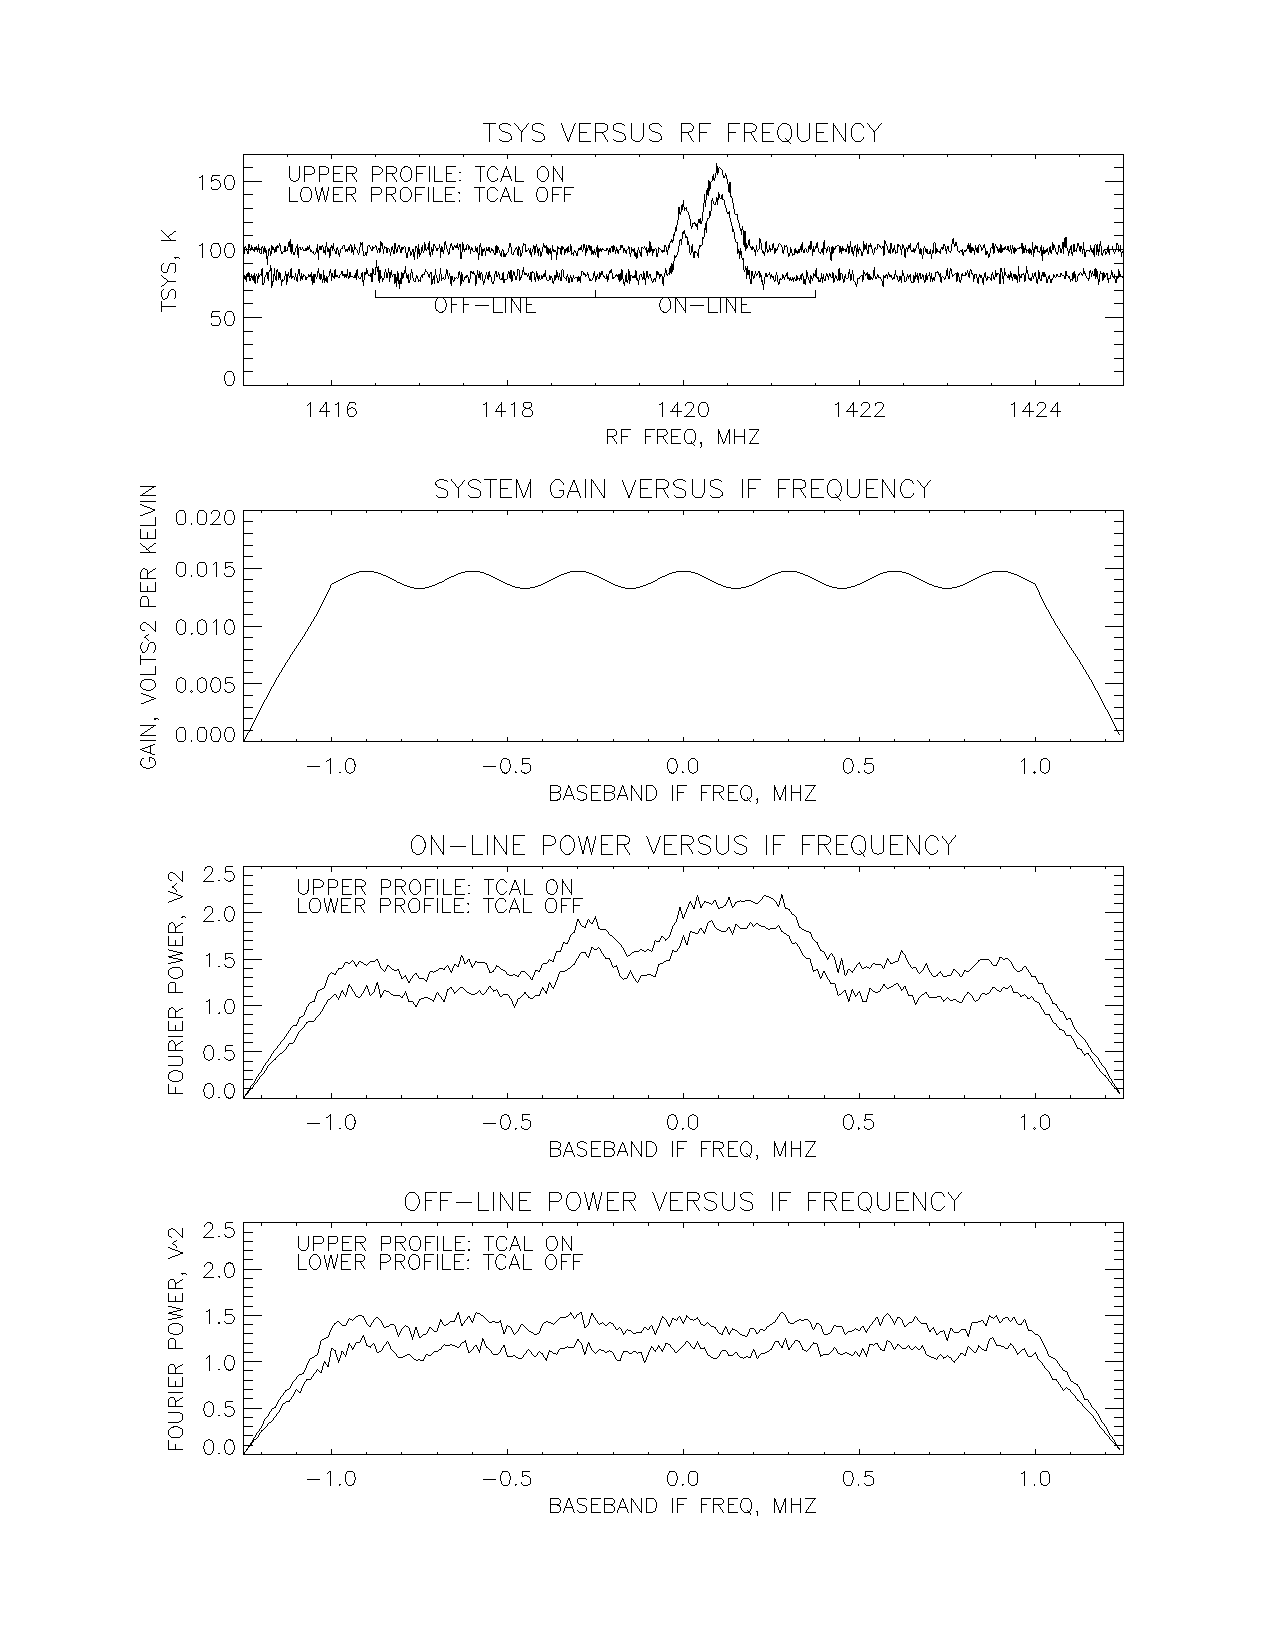
\includegraphics[width=5in]{bumpmountain_cal.pdf}
%\end{center}

\caption{ An HI line profile and its system contaminates, which must be
removed by calibration. \label{bumpmountain_cal}}

\end{figure}

	Let's take some time to analyze Figure \ref{bumpmountain_cal}.

\subsection{The Top Panel}

	The top panel shows the {\it actual} system temperature
$T_{sys}(\nu)$ over a fairly wide bandwidth for two conditions, one with
the noise diode on (``cal on'') and one with cal off. The cal adds 20 K
to the system temperature.

	The top panel shows noise on the spectrum. In fact, of course,
the system temperature itself has no noise on it; it's our {\it
measurement} procedure that {\it introduces} the noise. As we discuss
elsewhere, the r.m.s.\ noise in the system temperature for each channel
$\Delta T_{sys}$ is approximately

\begin{equation}
\Delta T_{sys} = { T_{sys} \over \sqrt{ \Delta \nu \tau}}
\end{equation}

\noindent where $\Delta \nu$ is the frequency width of each channel and
$\tau$ is the integration time. The product $\Delta \nu \tau$ is known
as the time-bandwidth product. Note that the noise decreases as $1 \over
\sqrt{\tau}$. The noise level on the top panel of Figure 1 is what a
perfect system would achieve with a time-bandwidth product of about
1000. For the HI line's typical frequency resolution of 5 kHz, that's
$\tau = 0.2$ sec. 

	The {\it system temperature} $T_{sys}(\nu)$ is a measure of the
total power of the system. There are two types of system temperature.
One is independent of frequency, and is usually called {\it continuum},
meaning that there is no structure with frequency. The other is
frequency-dependent, and because the spectral line is probably the
dominant contributor this is usually called {\it line}. So we have
\begin{enumerate}

	\item {\it Continuum contributions}. For these there is no
frequency dependence, so so we drop the parenthetical $(\nu )$ and
write, for example, $T_{rcvr}$ instead of $T_{rcvr}(\nu)$. Contributors
include \begin{enumerate}

	\item The {\it receiver temperature} $T_{rcvr}$. This is the
portion contributed by the electronics. In a well-designed system all of
this noise comes from the first amplifier in the chain, the one that is
connected directly to the antenna. For the case of Figure
\ref{bumpmountain_cal}, $T_{rcvr} \sim 70$ K.
s
	\item The {\it continuum antenna temperature} $T_{ant, cont}$,
which comes primarily from synchrotron radiation in the Galaxy. Galactic
ionized gas and the Earth's atmosphere contribute to what is usually a much
smaller extent. For typical positions in the sky, this amounts to about
10 K. 

\item For the case of Figure \ref{bumpmountain_cal}, $(T_{rcvr} + T_{ant,
  cont}) = 80$ K. This is reflected in the top panel. 

	\item The {\it cal temperature} $T_{cal}$, which is noise
generated by a noise diode. We switch this on and off to calibrate the
intensity scale. Because this adds to the system temperature, and thus
$\Delta T_{sys}$, we want to obtain our data with the cal turned off.
Figure \ref{bumpmountain_cal}, $T_{cal} = 20$ K. This is reflected in
the top panel.

\end{enumerate}

\item {\it Spectral line contributions}. For our work, this is the HI
line, so we have as the sole contributor \begin{enumerate}

	\item The {\it spectral antenna temperature} $T_{ant, HI}(\nu)$,
which maxes out at perhaps 30 K for the 21-cm line as seen with our
broad-beam horn.

\end{enumerate}
\end{enumerate}

	The total system temperature is the sum. Thus, when the cal is
off, we have

\begin{mathletters}
\begin{equation} \label{tsyscalon}
T_{sys}(\nu) = T_{rcvr} + T_{ant, cont} + T_{ant, HI}(\nu) = 
	T_{sys}  + T_{ant, HI}(\nu) 
\end{equation}

\noindent The totality of the frequency independent portion, $T_{rcvr} +
T_{ant,cont}$ is usually referred to as the {\it system temperature}
$T_{sys}$\footnote{Strictly speaking, the system is the sum of {\it all}
contributions, even including $T_{ant,HI}$, and is thus frequency
dependent.}. When the cal is on we have

\begin{equation} \label{tsyscaloff}
T_{sys}(\nu) = T_{rcvr} + T_{ant, cont} + T_{cal} + T_{ant, HI}(\nu) = 
	T_{sys}  + T_{cal} + T_{ant, HI}(\nu) 
\end{equation}
\end{mathletters}

	The top panel shows these two conditions, cal on and cal off. It
also shows the nonzero system temperature off of the line; the line adds
to what's already there in the continuum. The only way to know how much
the line contributes to $T_{sys}(\nu)$ is to observe a large enough
bandwidth so that you are sure that the line has dropped to zero.
Sometimes ``being sure'' is not so easy (see \S \ref{figure3}).

\subsection{The Second Panel}

	The total system power, which consists not only of $T_{ant}$ but
also $T_{rcvr}$, goes through our receiver system, which consists of
amplifiers, mixers, filters, and cables connecting them all. The system
spoils the signal because the system has a frequency dependent gain.
This gain multiplies the system temperature. The second panel shows this
gain versus IF frequency.

\subsubsection{ The frequency dependence of gain occurs at IF}

	The second panel exhibits a typical frequency-dependent gain
$G(\nu)$. This requires a bit of explanation. We make the assumption
that we can split the gain into two components, one being before the
first mixer [and thus at RF: $G_{RF}(\nu)$] and one after [and thus at
IF: $G_{IF}(\nu)$]. We assume that the gain {\it before} the first mixer
has {\it no} frequency dependence, so that $G_{RF}(\nu) = G_{RF}$. We
assume that {\it only} the components {\it after} the first mixer
exhibit frequency dependence. This assumption allows us to write 

\begin{equation}
G(\nu) = G_{RF} \cdot G_{IF}(\nu)
\end{equation}	

	Again, we emphasize the fact that we assume $G(\nu)$ depends
{\it only on the IF frequency} and is is {\it independent of RF
frequency}. This means that, in the power spectrum we derive using the
FFT, $G(\nu)$ is a function of the frequency index $j$; and,
additionally, $G(\nu)$ does {\it not} depend on the LO frequency. In
radio astronomy jargon, $j$ is called the {\it channel number}. 

	Our assumption means that we can write $G_j$ in place of
$G(\nu)$, and $G_j$ completely specifies the gain no matter what the LO
frequency is. The channel number refers explicitly to the IF frequency,
not the RF frequency, because it is computed from the baseband signal.
In the example of Figure \ref{bumpmountain_cal}, the IF frequency runs
from --1.25 to +1.25 MHz and $j$ runs from, we shall say, 0 to $2J-1$;
the total number of channels is $2J$. 

	Realizing that $j$ refers to IF frequency, and that the gain
$G(\nu)$ depends only on IF and not on RF frequency, we can define for
the gain

%\begin{mathletters}
\begin{equation}
G_j \equiv G(\nu)
\end{equation}

\subsubsection{The contributors to $G_j$ }

	There are two primary contributors to the gain $G_j$.  The most
important is the overall shape, which is determined by the base-band
filter; in our case this is a smooth low-pass filter having a gradual
falloff at the upper edge; filters in many radioastronomical systems are
{\it much} less benign (with shapes that are anything but smooth).

	Less prominent, but nevertheless important, is wiggles caused by
other effects. Here we show sinusoidal wiggles, which  are produced by
imperfect VSWR's produced by impedance mismatch of the various system
components. Sometimes there are additional artifacts produced by
God-knows-what.

%\section{Determining the calibrated spectrum}

%\subsection{The spectral shape}	

\subsection{The third and fourth panels}

	We can also use the subscript $j$ for the measured power
$P(\nu)$, but here we must realize that the $\nu$ in $P(\nu)$ refers to
RF frequency. The RF frequency, in turn, depends on the LO frequency, so
we need an additional specification for the central RF frequency. Here
we use the superscripts $OFFLINE$ and $ONLINE$, so we write

\begin{equation}
P_j^{OFFLINE} \equiv P(\nu) \ for \ offline \ spectrum
\end{equation}

\begin{equation}
P_j^{ONLINE} \equiv P(\nu) \ for \ online \ spectrum
\end{equation}

\noindent See Figure \ref{bumpmountain_cal} for the offline and online
spectra.

	The system gain $G_j$ multiplies the system temperature, so the
measured output spectrum $P_j$ is just

\begin{equation}
P_j = G_j T_{sys}(\nu)
\end{equation}

	Panels three and four show $P_j$ for the 2.5 MHz bandwidth segments
centered on the line (the $ONLINE$ spectrum) and off the line. If there
were no noise, the $OFFLINE$ spectrum would have exactly the same shape
as the second panel because it multiplies the frequency-independent system
temperature $T_{sys}$:

\begin{equation} \label{basiceqn} 
P_j^{OFFLINE} = G_j T_{sys} 
\end{equation}

\section{FIGURE \ref{bmp_cal}: OBTAINING THE CALIBRATED SPECTRUM
$T_{sys}(\nu)$ FROM THE MEASUREMENTS}

	Our goal is to obtain $T_{ant, HI}(\nu)$. To this end we obtain
three measurements: \begin{enumerate}

\item The ONLINE, CALOFF measurement, which gives the instrumental
response times the HI line

\begin{mathletters} \label{basiceqns}
\begin{equation} \label{ponline}
P_j^{ONLINE, CALOFF} = G_j (T_{sys} + T_{ant, HI}(\nu))  \ ;
\end{equation}

\item The OFFLINE, CALOFF measurement, which gives the instrumental
response by itself

\begin{equation} \label{poffline}
P_j^{OFFLINE, CALOFF} = G_j (T_{sys} ) \ ;
\end{equation}

\item The OFFLINE, CALON measurement, which gives us our intensity
calibration. $T_{cal}$ is our ultimate intensity calibration: it is the
only known temperature in this set of measurements. 

\begin{equation} \label{pcalon}
P_j^{OFFLINE, CALON} = G_j (T_{sys} + T_{cal}) \ .
\end{equation}
\end{mathletters}
\end{enumerate}

	We need to manipulate these measurements to calculate the best
estimate of our desired quantity $T_{ant,HI}(\nu)$.  There are two ways
to obtain this calibrated spectrum. One is straightforward and not so
good; the other is less straightforward and much better.

\begin{figure}[p!]
%\begin{center}
%\leavevmode
%\epsfxsize=5in
%\epsffile{bmp_cal.ps}
\centering
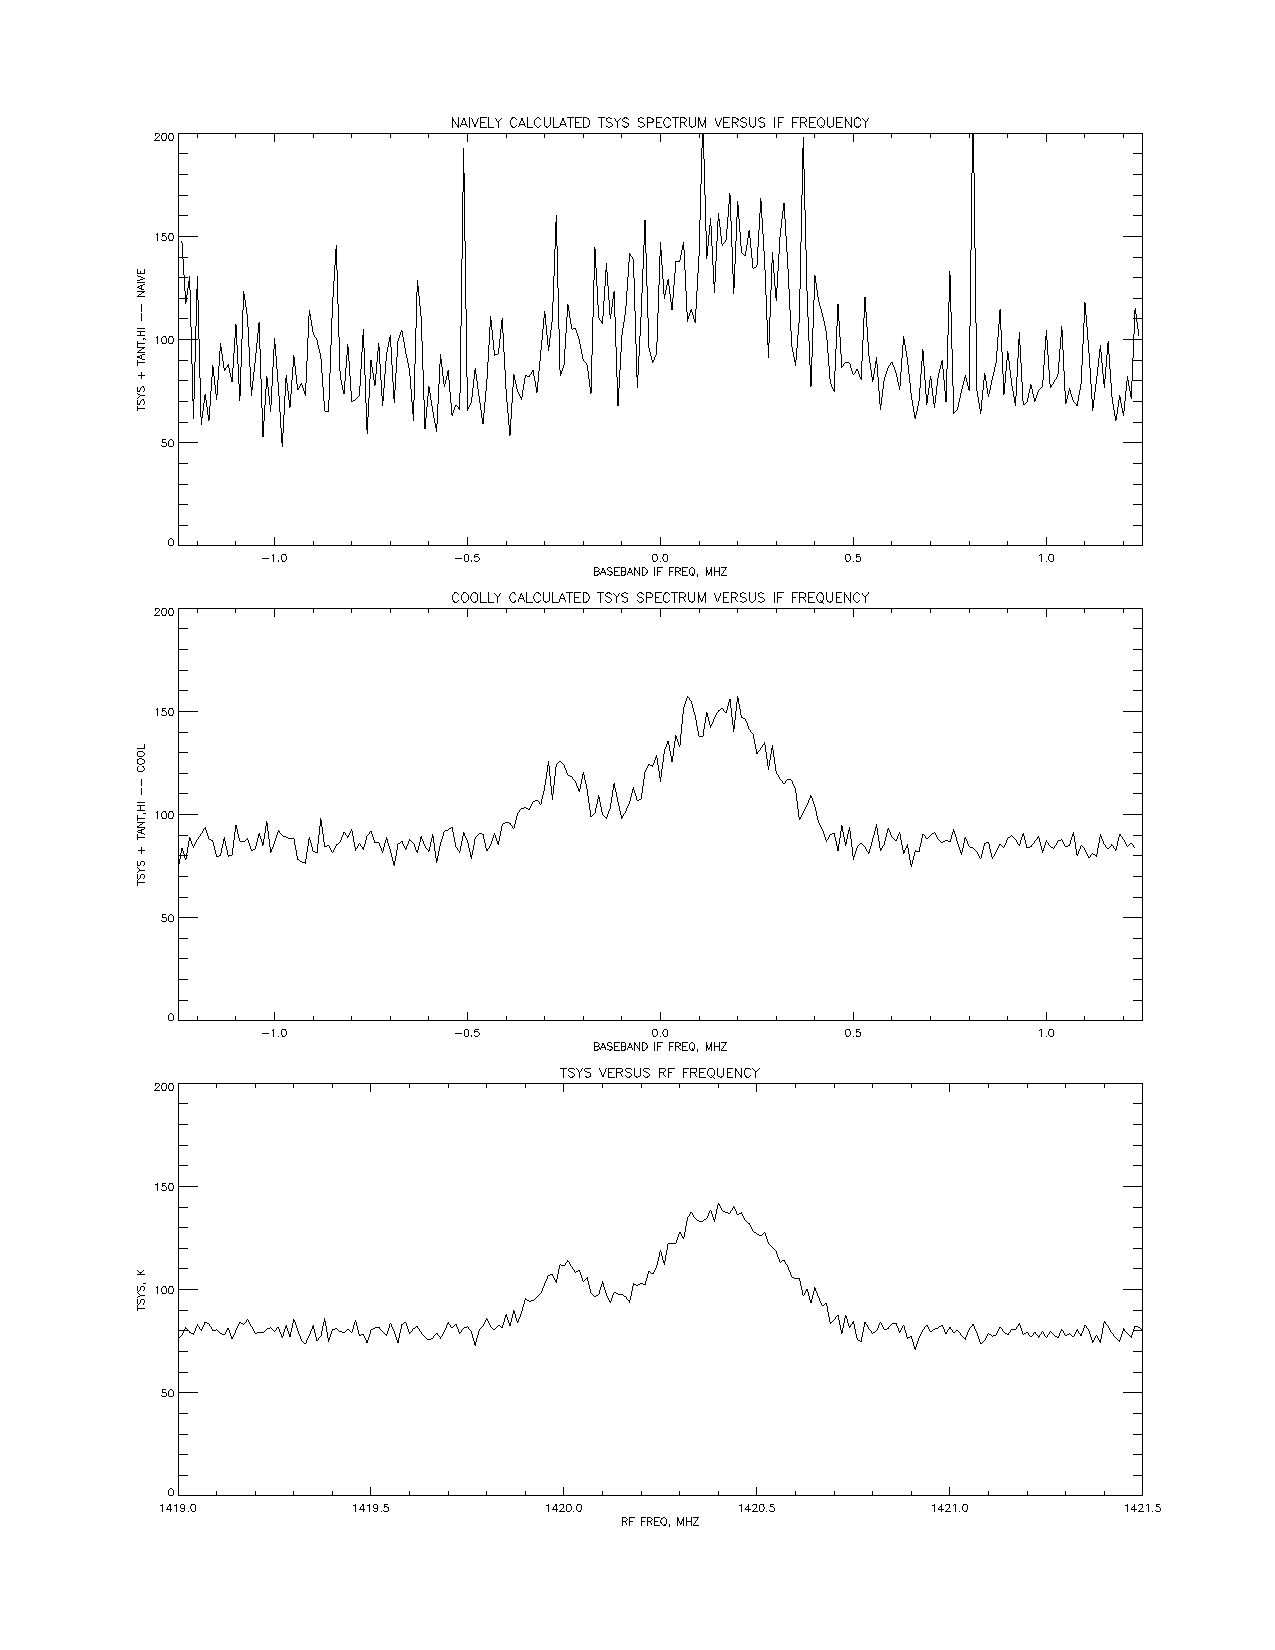
\includegraphics[width=5in]{bmp_cal.pdf}
%\end{center}

\caption{ Top two panels: two different reduction techniques: na\"ive
and cool. Bottom panel: the ON-LINE spectrum from the top panel of
figure \ref{bumpmountain_cal} \label{bmp_cal}}

\end{figure}

\subsection{The n\"aive method}

	With this method, we use the cal in a very straightforward way.
First, we use equations \ref{poffline} and \ref{pcalon}, with $CALON$ and
$CALOFF$,  and take the difference to give

\begin{mathletters}
\begin{equation} \label{naive1}
P_j^{OFFLINE,CALON} - P_j^{OFFLINE,CALOFF} =  G_j T_{cal}
\end{equation}

\noindent (Actually, the $CALON-CALOFF$ spectra can be done either $ONLINE$
or $OFFLINE$; all temperatures but $T_{cal}$ drop out in the difference).
This equation provides $G_j$ on a channel-by-channel basis:

\begin{equation} \label{naive2}
G_j = {P_j^{OFFLINE,CALON} - P_j^{OFFLINE,CALOFF} \over T_{cal}}
\end{equation}
\end{mathletters}

\noindent Knowing $G_j$, we can apply it to the $ONLINE,CALOFF$ spectrum
in equation \ref{ponline}. Making this substitution, we obtain

\begin{equation} \label{naive3}
T_{sys} + T_{ant, HI}(\nu) = \left[ {P_j^{ONLINE, CALOFF} \over 
P_j^{OFFLINE,CALON} - P_j^{OFFLINE,CALOFF}} \right] \left[ T_{cal} \right]
\end{equation}

\noindent We show this result in the upper panel of Figure \ref{bmp_cal}.
We see the line, but it's very {\it noisy}. That is, there is a lot of
channel-to-channel noise. This occurs because the gain of each channel
is determined individually and independently. 

\subsection{The cool method}

	The cool method very much reduces the channel-to-channel noise
by being clever in the determination of the channel gains. Let's begin
by doing some elementary rewriting of equations \ref{basiceqns}. First
rewrite equation \ref{ponline} to explicitly provide our desired quantity
$T_{sys} + T_{ant,HI}(\nu)$,

\begin{mathletters}

\begin{equation} \label{ponline1}
T_{sys} + T_{ant, HI}(\nu) = {P_j^{ONLINE, CALOFF} \over G_j}   \ .
\end{equation}

\noindent From this equation it is clear that if we know $G_j$ we know
$T_{sys} + T_{ant, HI}(\nu)$. Now rewrite equation \ref{poffline} to
explicitly give $G_j$

\begin{equation} \label{cool1}
G_j = {P_j^{OFF-LINE} \over T_{sys} }
\end{equation}

\end{mathletters}

\noindent From these two equations it is clear that if we know the
constant $T_{sys}$, we know $G_j$. This might seem like a tautology, but
it's not. Even if we don't know $T_{sys}$, $P_j^{OFF-LINE}$ tells us the
{\it shape} of $G_j$---and $P_j^{OFF-LINE}$ has little noise. All we
lack is the multiplicative constant $T_{sys}$, which is a constant,
independent of frequency. To be explicit, combine equations
\ref{ponline1} and \ref{cool1} and eliminate $G_j$, which gives

\begin{equation} \label{cool2}
T_{sys} + T_{ant, HI}(\nu) = 
\underbrace{\left[ {P_j^{ONLINE, CALOFF} \over P_j^{OFFLINE, CALOFF}} 
\right]}_{the shape} \cdot
\underbrace{ T_{sys}}_{scaling factor}   
\end{equation}

\noindent It remains to determine $T_{sys}$ so we can
get not only the shape, but the proper ``vertical scale''. 

	We get $T_{sys}$ from the cal as follows. First, on a
channel-by-channel basis we would have (by combining equations
\ref{poffline} and \ref{pcalon})

\begin{equation} \label{cool3}
T_{sys,j} = {P_j^{OFFLINE,CALOFF} \over 
	P_j^{OFFLINE,CALON} - P_j^{OFFLINE,CALOFF} } T_{cal}
\end{equation}

\noindent This gives us $2J$ different values for $T_{sys}$. Now realize
that $T_{sys}$ is independent of frequency (by assumption; in practice,
this assumption is usually very good). With this, we can use the full
bandwidth in both the numerator and denominator, 

\begin{equation} \label{cool3a}
T_{sys} =  {\sum_{j=0}^{j=2J-1} P_j^{OFFLINE,CALOFF} \over 
             \sum_{j=0}^{j=2J-1} \left(
P_j^{OFFLINE,CALON} - P_j^{OFFLINE,CALOFF} \right) } T_{cal} \ ,
\end{equation}

\noindent and we insert this {\it single} number into equation
\ref{cool2}. That is, we can write (in direct comparison to equation
\ref{naive3})

\begin{small}
\begin{equation} \label{cool4}
T_{sys} + T_{ant, HI}(\nu) =
\underbrace{ \left[ {P_j^{ONLINE, CALOFF} \over P_j^{OFFLINE, CALOFF}}
\right] }_{the shape}
\underbrace{ \left[ 
{\sum_{j=0}^{j=2J-1} P_j^{OFFLINE,CALOFF} \over 
             \sum_{j=0}^{j=2J-1} \left(
P_j^{OFFLINE,CALON} - P_j^{OFFLINE,CALOFF}  \right) } \right] T_{cal}}
	_{T_{sys}:a \ constant,\ inpdendent \ of \ j}
\end{equation}
\end{small}

\noindent We show this result in the middle panel of Figure
\ref{bmp_cal}. Note the much smaller noise!


\subsection{Why so cool?}

	Why is the cool method so cool? Because there's less noise! The
reason is clear when we compare the ratios of the various $P_j$
combinations between equations \ref{naive3} and \ref{cool4}: everything
is the same in these equations except that, in the cool method, we
average ${P_j^{OFFLINE,CALOFF} \over  P_j^{OFFLINE,CALON} - P_j^{OFFLINE,CALOFF}}$ over
channels ($j$). This quantity has lots of channel-to-channel noise
because the denominator contains a difference between two measured
spectra; by replacing its channel-by-channel noise fluctuations with the
channel-independent average, we get rid of this channel-to-channel noise
component. 

	You can look at it another way: the {\it shape} is given by the
lower-noise ratio $\left[ {P_j^{ONLINE, CALOFF} \over P_j^{OFFLINE, CALOFF}} 
\right]$; the {\it scaling} is given by $T_{sys}$, which in turn depends
on $T_{cal}$. In contrast, for the n\"aive method, both the shape and
the scaling are given by $T_{sys,j}$.

	There is more, though. We have implicitly assumed that the
integration times for $CALOFF$ and $CALON$ spectra are identical. But we
don't want to spend (``waste'') any more time than needed on calibrating
the intensity scale. This means we'd like to spend only a short time on
the $CALON$ spectrum, meaning that it will have increased noise. This,
in turn, will increase the noise in $P_j^{CALON} - P_j^{CALOFF}$
compared to what it would be if we had equal time. This would make the
n\"aive method {\it even worse} than the top panel of Figure
\ref{bmp_cal}.

\subsection{If it's so cool, why\dots}

	Look at the bottom panel of Figure \ref{bmp_cal}. This is the
original spectrum from the top panel of Figure \ref{bumpmountain_cal}.
And it has less noise than the cool method! If the cool method is so
cool, why can't it recover the original smaller noise level?

	The answer lies in the necessity to remove the effects of $G_j$.
This, in turn, requires combining $P_j^{ONLINE, CALOFF}$, which is the
ON-LINE spectrum from the top panel of Figure \ref{bumpmountain_cal},
with the OFF-LINE spectrum from that same panel. Each has noise, and
both noises contribute to the final result.

\section{ERROR PROPAGATION}

	This leads us to consider the way in uncertainty (or error,
or noise), propagates when we arithmetically combine quanties. This is
treated in books on statistics. Probably the best introductory text is
Taylor's {\it An Introduction to Error Analysis}. In chapter three he
discusses this propagation. 

	The basic rule is expressed in his equation 3.47. Suppose the
quantity $q$ is a function of $x$ and $y$, and the errors in $x$ and $y$
are $\delta x$ and $\delta y$. Then the error in $q$ is just

\begin{equation}
\delta q^2 = \left( {\partial q \over \partial x} \delta x \right)^2
 + \left( {\partial q \over \partial y} \delta y \right)^2
\end{equation}

\noindent One important thing to notice is that the errors add {\it
quadratically}. Another important thing to notice is the two most common
special cases: \begin{enumerate}

	\item For sums and differences, we have

\begin{mathletters}
\begin{equation} 
q = (x + y) \ \ {\rm OR} \ \ q = (x - y)
\end{equation}
\begin{equation} \label{sumprop}
\delta q^2 = \delta x^2 + \delta y^2
\end{equation}
\end{mathletters}

\noindent So the errors add quadratically, which makes sense. 

	\item For products and ratios, we have
 
\begin{mathletters}
\begin{equation} \label{productprop}
q = xy \ \ {\rm OR} \ \ q = {x \over y}
\end{equation}
\begin{equation} \label{errorproduct}
\left({\delta q \over q}\right)^2= \left( \delta x \over x \right)^2 + \left( \delta y \over y \right)^2 
\end{equation}
\end{mathletters}

\end{enumerate}

\noindent The generatlization to more variables than just $x$ and $y$
should be obvious. Let's apply these rules to our situation:

\subsection{ Application of equation \ref{sumprop} for {\it averages}}

	When we take a long integration and combine many spectra, we are
taking the sum of $N$ spectra, each with its independent error, and
dividing by $N$ to get the average. Suppose each spectrum has the same
error $\Delta T_{sys}$ (by ``same'', we mean {\it statistically} the
same, not {\it identically} the same!). From equation \ref{sumprop},
the error in the {\it sum} is just

\begin{mathletters}
\begin{equation}
(error \ in \ sum)^2 = \left[ \sum_0^{N-1} (\Delta T_{sys,n})^2 \right]
=	N (\Delta T_{sys})^2
\end{equation}

\noindent The average is the sum divided by $N$, the square of the
average is the square of the sum divided by $N^2$. Similarly, the error
in the {\it average} is just that in the sum divided by $N^2$, i.e.

\begin{equation} 
(error \ in \ average)^2 = {(\Delta T_{sys})^2 \over N}
\end{equation}
 
\noindent or

\begin{equation} 
(error \ in \ average) = { error \ in \ each \ measurement  \over \sqrt{N}}
\end{equation}
\end{mathletters}

	This illustrates the famous, and almost general, rule that the
noise decreases as the square root of the number of times that a
measurement is repeated. ``The noise decreases as root $N$''. In our
case this rule is fulfilled by the noise decreasing as $1 \over
\sqrt{\tau}$. 

\subsection{ Application of equation \ref{productprop} for the cool
method}

	Let's again write equation \ref{cool2}, but for brevity replace 
$T_{sys} + T_{ant, HI}(\nu)$ by $T_{sys}(\nu)$, where we incorporate the
frequency-independent $T_{sys}$ and frequency-dependent $T_{ant,
HI}(\nu)$ into a single frequency-dependent system temperature
$T_{sys}(\nu)$: 

\begin{equation} 
T_{sys}(\nu) = 
\underbrace{\left[ {P_j^{ONLINE, CALOFF} \over P_j^{OFFLINE, CALOFF}} 
\right]}_{the shape} \cdot
\underbrace{ T_{sys}}_{scaling factor}   
\end{equation}

\noindent If we apply equation \ref{errorproduct}, we get

\begin{equation}
\delta T_{sys}(\nu)^2 = 
\left[ \left( {\delta P_j^{ONLINE, CALOFF} \over P_j^{ONLINE,
CALOFF}} \right)^2 +  \left( {\delta P_j^{OFFLINE, CALOFF} \over P_j^{OFFLINE,
CALOFF}} \right)^2 \right] T_{sys}^2
\end{equation}

\noindent But the statistical properties of $P_j^{ONLINE, CALOFF}$ and
$P_j^{OFFLINE, CALOFF}$ are the same, so we find that

\begin{equation}
\delta T_{sys}(\nu)^2 = 2 
 \left( {\delta P_j^{ONLINE, CALOFF} \over P_j^{ONLINE,
CALOFF}} \right)^2 T_{sys}^2
\end{equation}

	In words: combining the two spectra $P_j^{ONLINE, CALOFF}$ and
$P_j^{OFFLINE, CALOFF}$, which have identical noise from the statistical
standpoint, increases the noise $\delta T_{sys}(\nu)^2$ by 2, or the
noise in $T_{sys}(\nu)$ by $\sqrt 2$. If you look carefully at the
bottom two panels of Figure \ref{bumpmountain_cal}, you will find that
this is the only difference. 

	There is no way around the introduction of this noise unless you
can generate a noise-free spectrum of $G_j$. In practice, nobody can do
this. 

	This brings up the question: because we have to measure both
$P_j^{ONLINE, CALOFF}$ and $P_j^{OFFLINE, CALOFF}$ and combine them, what
is the optimum ratio of time to spend on each? In particular, doesn't it
make sense to spend more time measuring the $ONLINE$ than the $OFFLINE$
spectrum? After all, that's where the signal is! 

	The somewhat surprising answer: given a fixed total integration
time, the best result is obtained by spending {\it equal time}. From the
discussion in this section, you know enough to prove this simple truth;
the proof is straightforward.

\section{FIGURE \ref{bmp_cal1}: REAL LIFE} \label{figure3}

\begin{figure}[p!]
%\begin{center}
%\leavevmode
%\epsfxsize=5in
%\epsffile{bmp_cal1.ps}
\centering
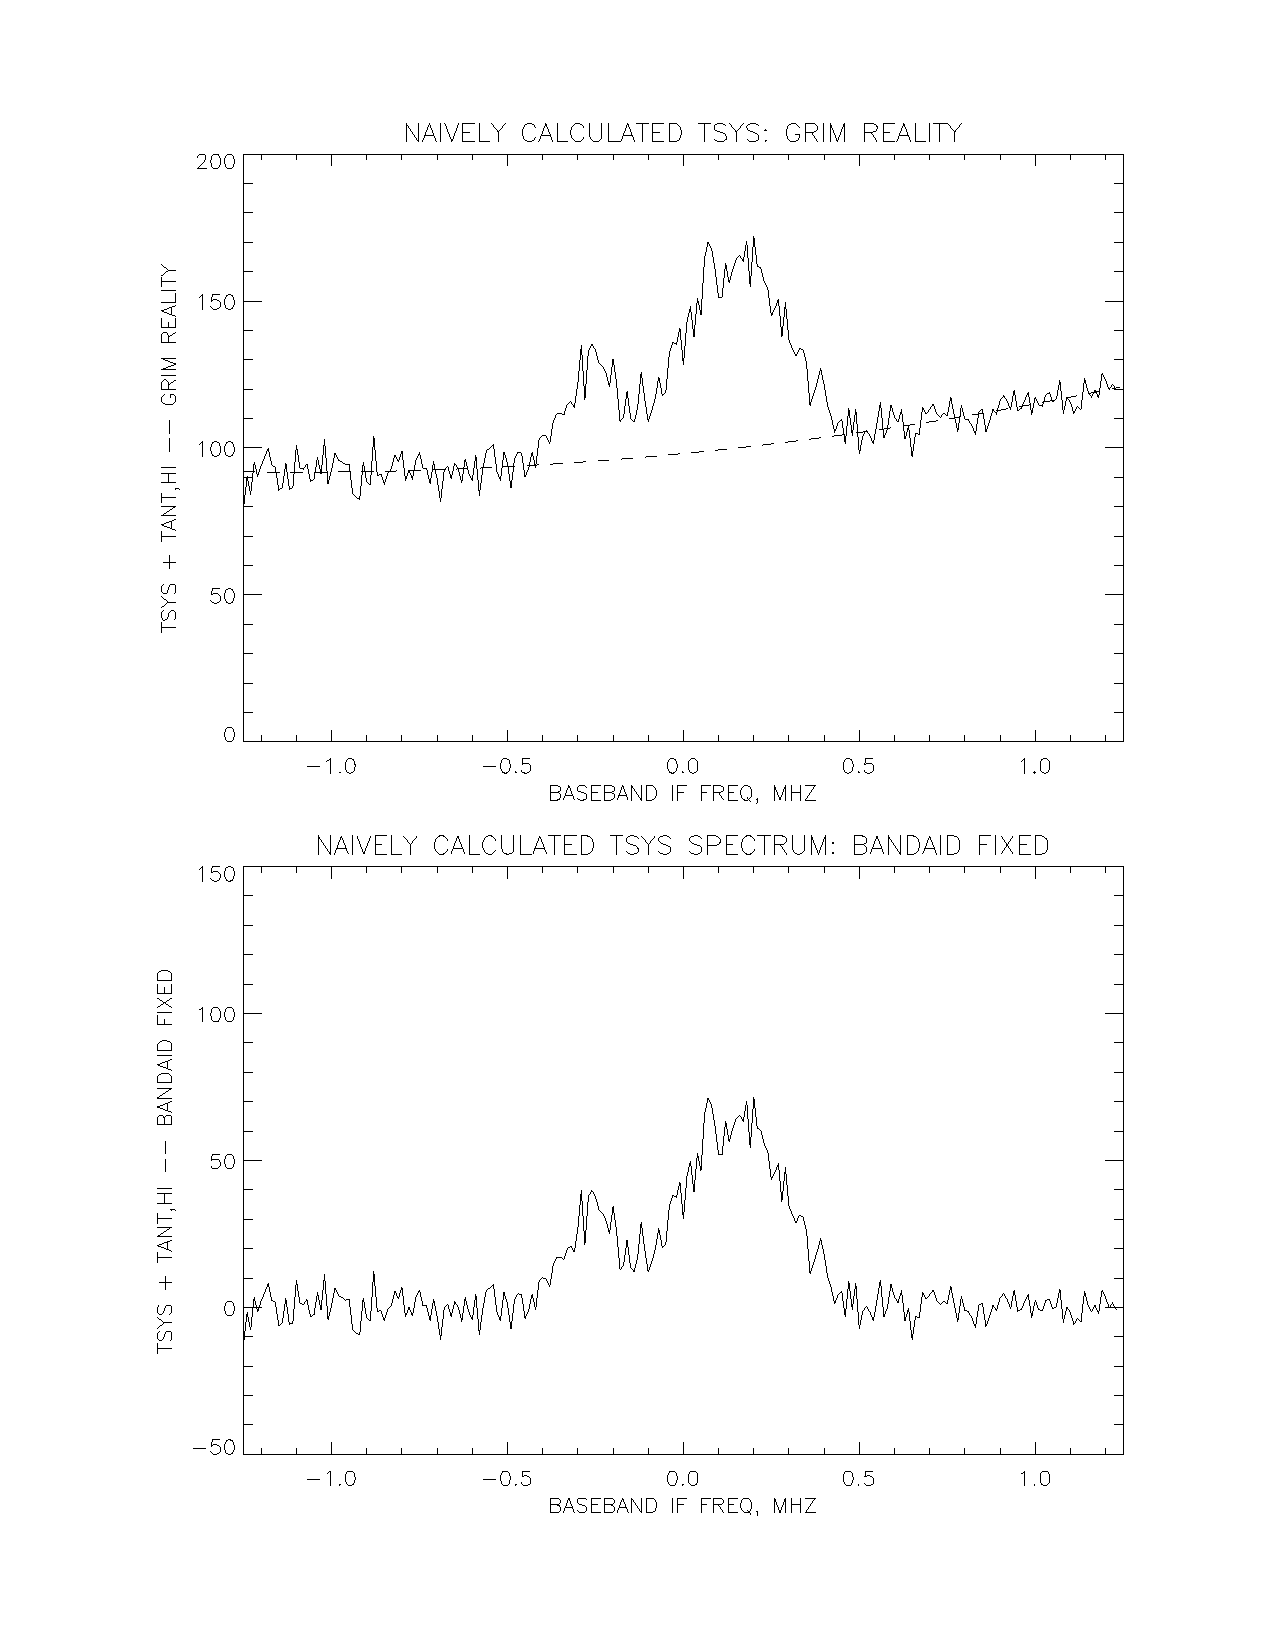
\includegraphics[width=5in]{bmp_cal1.pdf}
%\end{center}

\caption{ The grim reality in spectral line measurements. Departures
from our ideal assumptions produce curved, displaced baselines, shown in
the top panel. Fitting a polynomial baseline with least squares and
subtracting it produces the apparently perfect spectrum im the botom
panel. \label{bmp_cal1}}

\end{figure}

	In reality, the result from equation \ref{cool4} is imperfect
because it contains additional artifacts. These occur because our
assumptions are not completely correct. Specifically, $G_{RF}$ is not
{\it exactly} independent of frequency; neither is $T_{rcvr}$. The most
obvious result of these is to make the spectrum have a non-flat
``baseline''; the baseline is the part of the spectrum outside the line.
In other words, if there were no line, the spectrum would not be flat.
The top panel in Figure \ref{bmp_cal1} shows a typical ``baseline
problem''. 

	These baseline problems plague spectral line observers and there
is no bulletproof solution. Accordingly, one fits an empirical smooth
curve to the baseline (the off-line portions of the $ONLINE$ spectrum).
One usually does this with a polynomial least squares fit\footnote{Use
either my {\it polyfit} or IDL's {\it poly\_fit}.}. The
dashed line in the top panel of Figure \ref{bmp_cal1} shows this fit;
the bottom panel shows the result minus the fit, in which the curvy
baseline is removed. 

	This fixed-up profile looks good. The baseline fit automatically
subtracts out the system temperature, so we are left with the a 21-cm
line profile coming from a zero baseline. 

	However, this procedure camouflages possible discoveries! For
example, in the top panel of Figure \ref{bmp_cal1} the whole spectrum is
displaced upwards relative to the ideal one in the bottom panel of
Figure \ref{bmp_cal}. Is this upward displacement an artifact, {\it or
it is it real?} It could be that our line sits on top of a very broad,
weak line whose emission is removed by the baseline-fitting procedure!
But the baseline fit subtracts out all this, making the implicit
assumption that it's an artifact.

\end{document}
\end

